\section{Durchführung}
\label{sec:Durchführung}
Der Versuchsaufbau ist in Abbildung \ref{fig:aufbau} dargestellt.
\begin{figure}
  \centering
  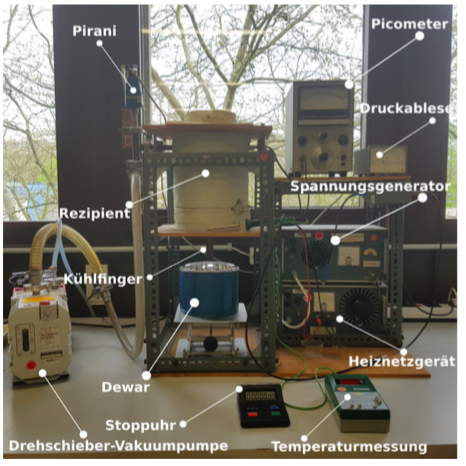
\includegraphics[width=10cm]{Aufbau.png}
  \caption{Versuchsaufbau \cite{skript}}
  \label{fig:aufbau}
\end{figure}
Die verwendete Probe ist $\ce{KBr}$, welches mit 0,005\% $\ce{Sr}$ dotiert ist.
Da dieser Kristall hygroskopisch ist, wird der Versuch im Vakuum durchgeführt, sodass vor Beginn des
Versuches der Rezipient zunächst bis auf einen Druck von etwa $\SI{1e-2}{\milli\bar}$
evakuiert wird. \\
Da das Feld über eine Zeit angelegt werden muss, welche lang ist gegenüber der Relaxationszeit,
wird die Probe zunächst durch die Heizspannung auf $\SI{320}{\kelvin}$ erwärmt, da hier die Relaxationszeit
kürzer ist als bei tieferen Temperaten. Ist diese Temperatur erreicht wird der Kondensator
mit der maximal möglichen Spannung von $\SI{950}{\volt}$ aufgeladen und für eine Zeit von
etwa $\SI{900}{\second}$ so belassen, damit sich ausreichend Dipole entlang des Feldes ausrichten.
Anschließend wird das Dewar-Gefäß mit flüssigem Stickstoff befüllt und so positioniert,
dasss er Kontakt mit dem Kühlfinger hat, sodass die Probe abkühlt. Hat diese eine Temperatur
von $\SI{210}{\kelvin}$ erreicht wird der Kondensator für etwa 5 Minuten kurugeschlossen, damit alle
Ladungen abfließen und kein äußeres Feld mehr vorhanden ist. \\
Daraufhin wird das Picoamperemeter angeschaltet und der Strom beobachtet, solange bis sich ein
konstanter Wert eingestellt hat. Nun wird mithilfe des Heizstroms eine konstante Heizrate von etwa
$\SI{2}{\kelvin}$ pro Minute eingestellt und jede Minute ein Wertepaar aus Depolarisationsstrom
und Temperatur notiert. Während der Messung muss dabei der Strom immer wieder angepasst werden,
da auch die Wärmekapazität temperaturrabhängig ist. Die Messung wird bis zu einer Temperatur von etwa
$\SI{325}{\kelvin}$ durchgeführt und anschließend wird der gesamte Prozess für eine
zweite Heizrate von $\SI{1}{\kelvin}$ pro Minute wiederholt.
